\section{RLVR's Effect on Reasoning Capacity Boundary}
\label{sec:exp}

With the evaluation metrics for reasoning boundaries established, we now conduct a comprehensive evaluation of the base and RLVR models through extensive experiments.  
Our analysis is organized by task category, covering three representative domains: mathematics, code generation, and visual reasoning.
The overall experimental setup is summarized in~\cref{tab:exp-settings}.


\textbf{Evaluation Protocol.}
For sampling procedures for both base and RLVR models, we use a temperature of 0.6 and a top-$p$ value of 0.95, allowing a maximum generation of 16,384 tokens.
We also show the effect of different temperature settings in~\cref{fig:different_T}.
For evaluation of the base model, a common practice is to include few-shot examples in the prompt to guide the output~\cite{grattafiori2024llama3,yang2024qwen25,liu2024deepseekv3}.
However, to ensure a fair and unbiased comparison, we deliberately avoid using few-shot prompts for base models, eliminating any potential confounding effects on reasoning that might be introduced by in-context examples.
For evaluating both the base and RLVR models, we use the same zero-shot prompt as in RLVR training, or the default prompt provided by the benchmark, ensuring a consistent setup across both models.
Interestingly, although base models often produce unformatted or non-sensical responses without few-shot guidance, we observe that with sufficient sampling, they are still capable of generating correctly formatted outputs and successfully solving complex problems.
Prompt templates for training and evaluation are provided in~\cref{appendix:prompt}.


\subsection{RLVR for Mathematical Reasoning}
\label{sec:math}

\textbf{Models and Benchmarks.}
In math problems, models are required to generate a reasoning process (\ie, CoT) along with the final answer.
To ensure the robustness of conclusions, we experiment with multiple LLM families, primarily Qwen2.5 (7B/14B/32B base variants)~\cite{yang2024qwen25} and additionally LLaMA-3.1-8B~\cite{grattafiori2024llama3}.
We adopt RLVR models released by SimpleRLZoo~\cite{zeng2025simplerl}, which train zero-RL models using GRPO on GSM8K and the MATH training set, with correctness reward only, excluding any format-based reward.
We compare the pass@$k$ curves of base and zero-RL models on benchmarks of varying difficulty:
GSM8K~\cite{cobbe2021gsm8k}, MATH500~\cite{hendrycks2021math500}, Minerva~\cite{lewkowycz2022minerva}, Olympiad~\cite{he2024olympiadbench}, AIME24, and AMC23. 
Additionally, we include the RLVR model Oat-Zero-7B and DAPO-32B~\cite{liu2025oat, yu2025dapo}.
These two models are characterized by strong performance on the challenging AIME24 benchmark.
% These two models are characterized by strong performance on the challenging AIME24 benchmark, achieving an average of 43.4\% points, substantially higher than the base model's performance of below 10\%.



\textbf{The Effect of RLVR: Increased Likelihood of Correct Samples, Decreased Coverage of Solvable Problems.}  
As shown in~\cref{fig:math}, we consistently observe a contrasting trend between small and large $k$ values.  
When $k$ is small (\eg, $k = 1$, equivalent to average-case accuracy), RL-trained models outperform their base counterparts. This aligns with the common observation that RL improves performance, suggesting that RLVR makes models significantly more likely to sample correct responses.
% However, as $k$ increases to the tens or hundreds, base models consistently catch up with RL-trained models across all benchmarks and LLM families without exception. 
% Notably, the pass@$k$ curves of base models exhibit a steeper upward trend compared to their RL-trained versions. 
% Ultimately, the base model surpasses the RL-trained model at sufficiently large $k$, indicating that the coverage of solvable problems by the base model is broader than that of the RL-enhanced version.
However, as $k$ increases, with steeper curves, base models consistently catch up to and eventually surpass RL-trained models across all benchmarks, indicating their broader coverage of solvable problems.
For example, on the Minerva benchmark with a 32B-sized model, the base model outperforms the RL-trained model by approximately 9\% at $k = 128$, implying that it can solve around 9\% more problems in the validation set.  

We further examine RL models trained with Oat-Zero and DAPO. As shown in~\cref{fig:oat_aime}, although the RL model initially demonstrates a strong performance, nearly 30\% higher than the base model, it is eventually surpassed by the base model. 
Based on these results, we conclude that RLVR increases the likelihood of sampling correct responses at low $k$, but narrows the model's overall coverage. We further analyze the root cause of this phenomenon in~\cref{sec:pattern_analysis}.


\textbf{CoT Case Analysis.}
We present the correct CoTs sampled from the base model in~\cref{fig:AIME24_16_Base_Answer} and~\cref{fig:AIME24_24_Base_Answer}, manually selected from 2048 samplings for the hardest questions in AIME24. 
The responses from the base model tend to be long CoTs and exhibit reflective behavior, highlighting the strong reasoning ability inherent in the base model.



\textbf{Validity of Chain-of-Thought.}  
For mathematical problems, the common evaluation is based solely on the correctness of the final answer, with the risk of ``hacking''.  
To accurately reflect the reasoning ability boundary using pass@$k$, it is important to assess how many solved problems result from sampling genuinely correct CoTs, rather than from lucky guesses. Following~\cite{brown2024monkey}, we manually inspect all CoTs that led to correct answers to the most challenging solvable problems in the GSM8k dataset -- those with an average accuracy below 5\% but above 0\%.
The base model answered 25 such questions, with 24 containing \textit{at least one} correct CoT. Similarly, the RL-trained model answered 25 questions, 23 of which included \textit{at least one} correct CoT.
% These results suggest that even on the hardest questions in GSM8k, problem-solving primarily results from sampling valid reasoning paths rather than relying on lucky guesses, implying that pass@$k$ at large $k$ values can serve as a relatively accurate indicator of a model's reasoning boundary.  
We also manually check the CoTs for problems in the challenging AIME24 benchmark with an average accuracy below 5\%. Details can be found in~\cref{appendix:cot_aime24}.
The base model answered 7 such questions, with 5 out of 6 containing \textit{at least one} correct CoT (excluding one ambiguous case of correctness due to skipped reasoning steps). Similarly, the RL-trained model answered 6 questions, 4 of which included \textit{at least one} correct CoT.
These results suggest that the base model can sample valid reasoning paths to solve the problems.

% \textbf{Truly Pass@$k$ with Manually CoT Verification.} \textcolor{blue}{[TODO.]}


\vspace{-1mm}
\subsection{RLVR for Code Generation}

\begin{wrapfigure}{r}{0.3\textwidth}
\vspace{-3mm}
  \centering
   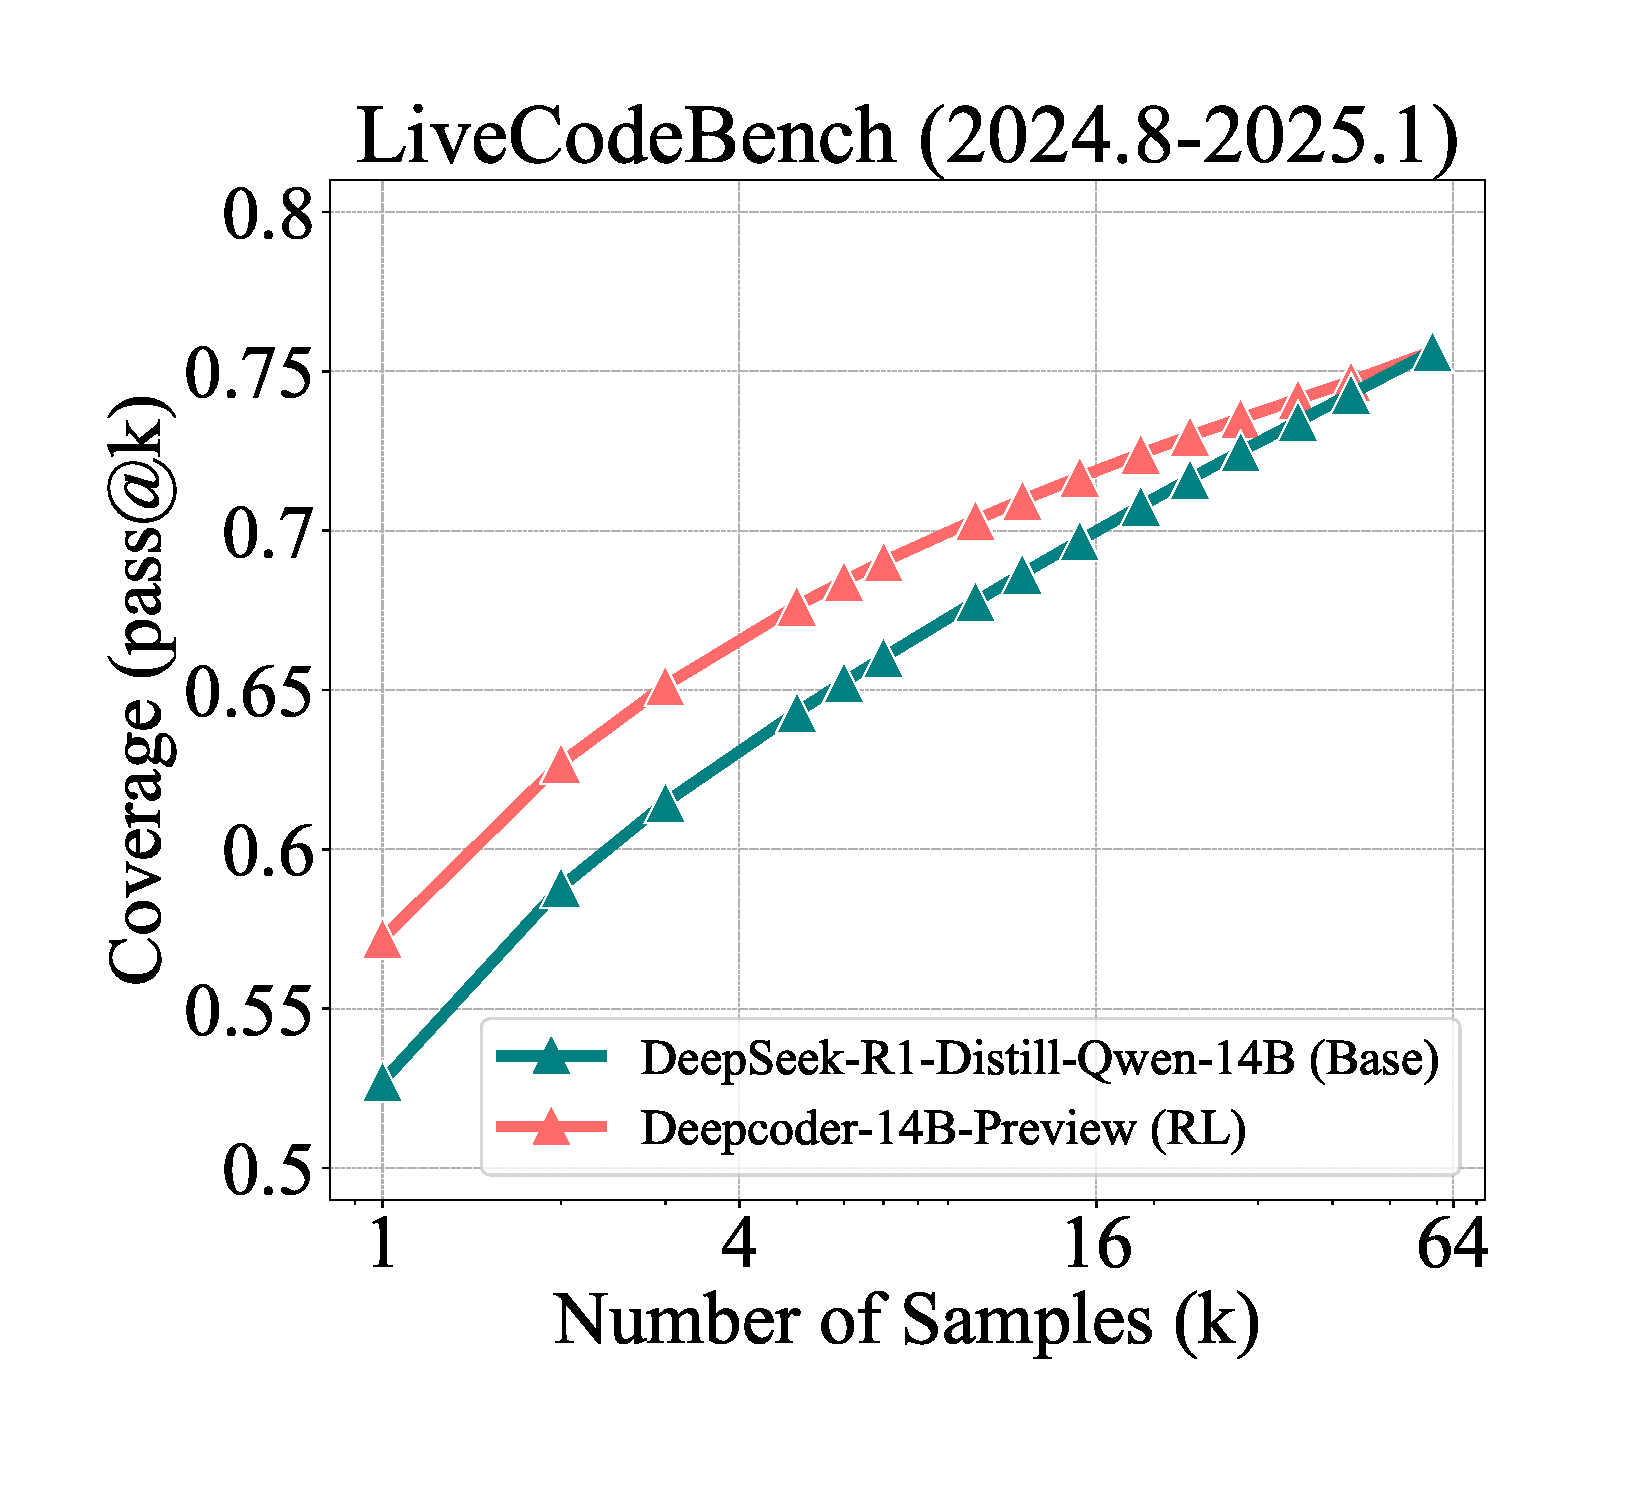
\includegraphics[width=0.3\textwidth]{tex/images/livecodebench_deepcoder.pdf}
\captionsetup{font={footnotesize}}
\vspace{-5mm}
 \caption{RLVR for Coding.}
  \label{fig:livecodebench}
\vspace{-4mm}
\end{wrapfigure}

\textbf{Models and Benchmarks.}
We adopt the open-sourced RLVR-trained model, CodeR1-Zero-Qwen2.5-7B~\cite{code-r1}, which trains zero-RL models on 12K LeetCode and TACO samples over 832 steps, based on Qwen2.5-7B-Instruct-1M~\cite{yang2025qwen25-1m}. 
% A binary correctness reward is provided by the compiler based on predefined test cases.
% For evaluation, Models are assessed on LiveCodeBench v5, comprising 880 problems that span from May 2023 to January 2025~\cite{jain2024livecodebench}, 
For evaluation, models are assessed on LiveCodeBench v5, comprising 279 problems that span from August 2024 to January 2025~\cite{jain2024livecodebench},
as well as HumanEval+ and MBPP+~\cite{evalplus}.
We also evaluate the most powerful open-source RLVR-trained coding LLM, DeepCoder-14B~\cite{deepcoder2025}, built on DeepSeek-R1-Distill-Qwen-14B. Here both models take 32k response length. Due to their high computational cost, we evaluate them only on LiveCodeBench as a representative benchmark.

\textbf{The Effect of RLVR.}  
Since passing all unit tests is nearly impossible to achieve by guesswork, pass@$k$ provides a reliable measure of a model's reasoning boundary.
As shown in~\cref{fig:livecodebench},~\cref{fig:coder_r1}, and~\cref{fig:code_and_visual} (left), the effects of RLVR on three code generation benchmarks exhibit trends that are highly consistent with those observed in mathematical benchmarks.  
% \textbf{The Effect of RLVR.}  
% As shown in~\cref{fig:livecodebench} and~\cref{fig:code_and_visual} left, the effects of RLVR on three code generation benchmarks exhibit trends that are highly consistent with those observed in mathematical benchmarks.  
% For instance, on LiveCodeBench, the original model achieves a pass@1 score of 23.8\%, while the RLVR-trained model achieves 28.1\%.  
% However, when sampling 128 times, approximately 50\% of coding problems can be solved by the original model, whereas only 42.8\% are solved by the RLVR model.  
% Furthermore, we observe that the slope of the original model's curve remains steep at $k = 128$, suggesting that pass@$k$ will continue to increase with larger $k$ values. In contrast, the curve for Code-R1 gradually converges.  
% This suggests that while RLVR shows improvements in single-sample performance, it results in a diminishing coverage boundary and has less potential than the original model.

% \textbf{Subset.}  

\vspace{-1mm}
\subsection{RLVR for Visual Reasoning} 


\textbf{Models and Benchmarks.}
In visual reasoning, models must jointly interpret visual and textual inputs to solve complex reasoning problems.
This has gained significant attention in the multimodal community since the rise of LLM reasoning~\cite{chen2025r1v,shen2025vlmr1,zheng2025easyr1}.
For our experiments, 
we select math within visual contexts as a representative task.
We use the EasyR1 framework~\cite{zheng2025easyr1} to train Qwen2.5-VL-7B~\cite{bai2025qwen25vl} on Geometry3K~\cite{lu2021geo3k}, and evaluate its visual reasoning capabilities on filtered MathVista-TestMini~\cite{lu2024mathvista} and MathVision-TestMini~\cite{wang2024mathvision}, where multiple-choice questions are removed.  
% Specifically, both MathVista and MathVision contain multiple-choice questions, which can be easily guessed through repeated sampling. Therefore, we remove multiple-choice questions from the evaluation.  
% After filterinlaigg, 460 problems remain out of 1000 in MathVista, and 114 problems remain out of 460 in MathVision.

\textbf{The Effect of RLVR.}  
As shown in~\cref{fig:code_and_visual} (right), the effects of RLVR on visual reasoning are highly consistent with those observed in math and coding benchmarks. This suggests that the original model has broader coverage of solvable questions even in multimodal tasks.

\textbf{Validity of Chain-of-Thought.}
Similarly, we manually inspect a subset of the most challenging problems, \ie those with an average accuracy below 5\%.  
% For each inspected problem, we review all CoTs that led to correct answers. 
We find that for both the original and RL models, 7 out of 8 problems have \textit{at least one} correct CoT.
These results support the validity of CoTs.
% These results suggest that even on the hardest questions in the filtered set, the increase of coverage primarily results from sampling valid reasoning paths, rather than relying on lucky guesses.


\begin{figure}
  \centering
  \begin{subfigure}[b]{0.495\textwidth}
    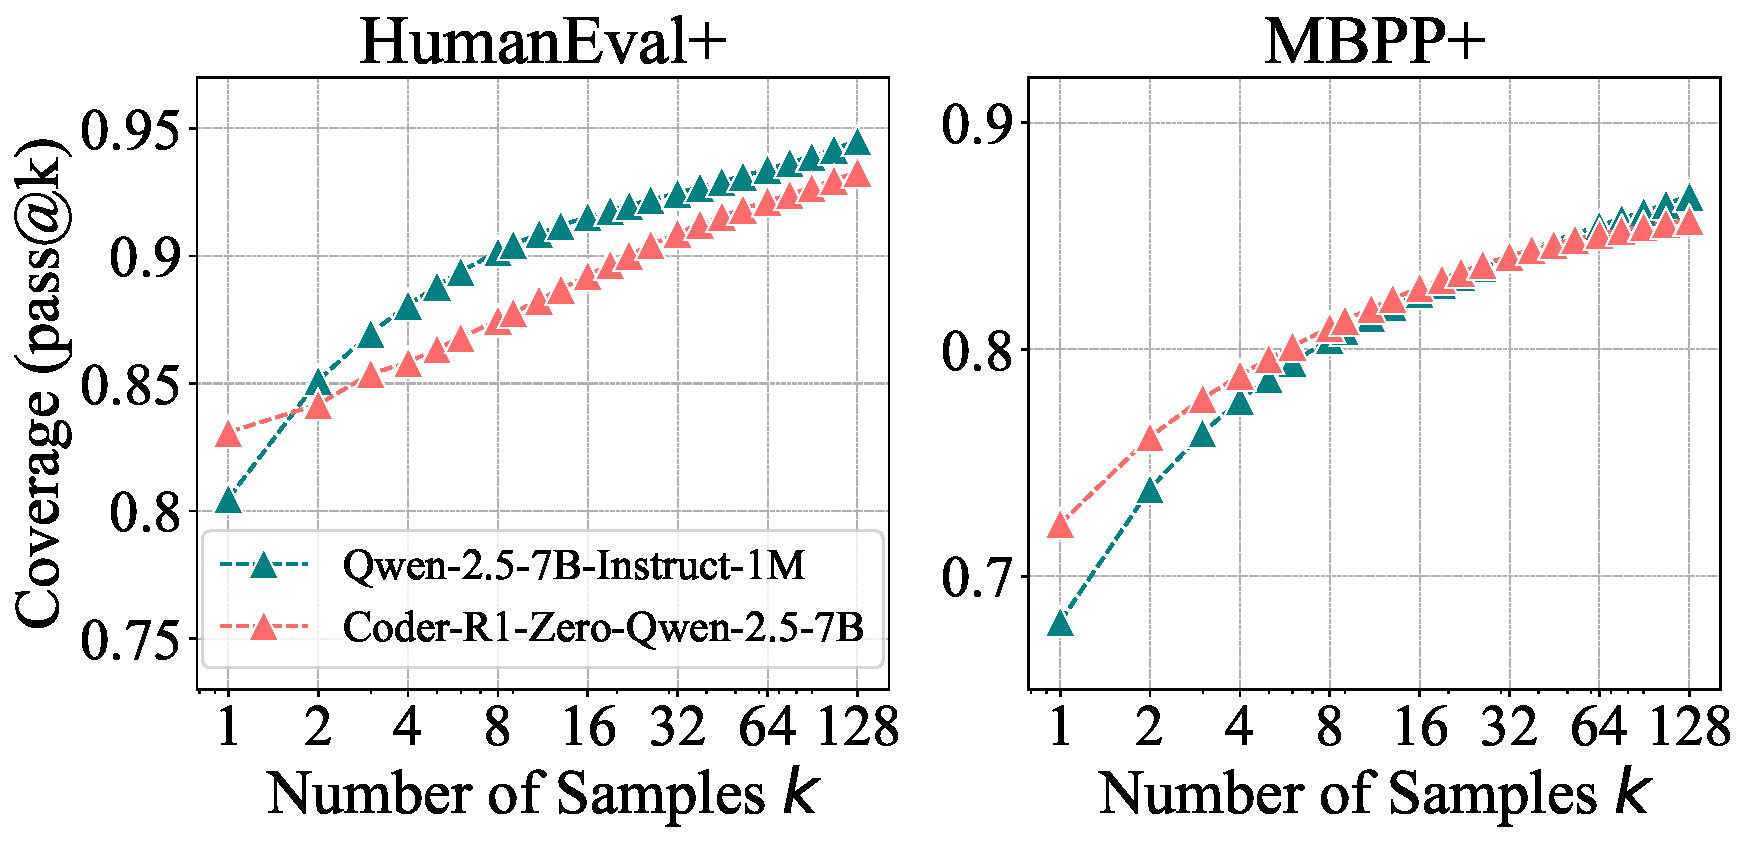
\includegraphics[width=\textwidth]{tex/images/code_qwen_7b_instruct_coverage.pdf}
    % \caption*{(a) code Generation.}
  \end{subfigure}
  % \hfill
  \begin{subfigure}[b]{0.495\textwidth}
    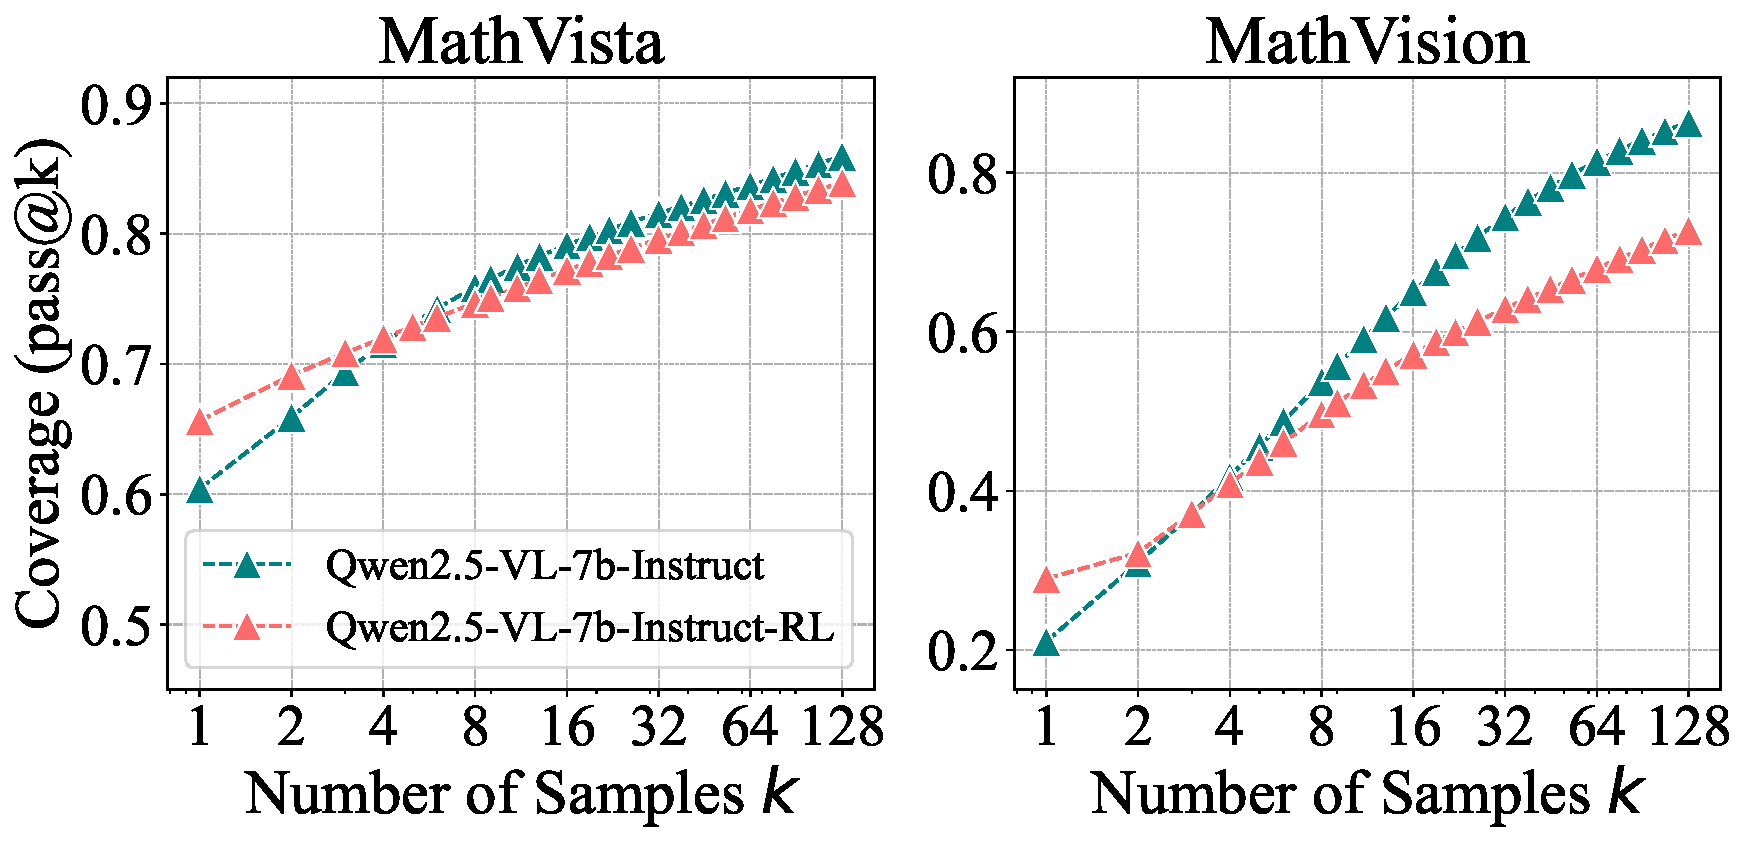
\includegraphics[width=\textwidth]{tex/images/qwenvl_7b_instruct_coverage_filter.pdf}
    % \caption*{(b) Visual Reasoning.}
  \end{subfigure}
\captionsetup{font={footnotesize}}
\caption{
Pass@$k$ curves of base and RLVR models.
\textbf{(Left)} Code Generation.
\textbf{(Right)} Visual Reasoning.
}
\label{fig:code_and_visual}
\vspace{-3mm}
\end{figure}


\section{Deep Analysis}
\label{sec:deep_analysis}

In this section, we conduct a deeper analysis of the effects of current RLVR training. We also highlight the distinct characteristics of distillation in comparison to RLVR. In addition, we design controlled experiments to examine the impact of different RL algorithms and design choices.

\subsection{Reasoning Paths Already Present in Base Models}
\label{sec:pattern_analysis}



\begin{wrapfigure}{r}{0.33\textwidth}
\vspace{-4mm}
  \centering
   \includegraphics[width=0.33\textwidth]{tex/images/simpleRL_his1.pdf}
\captionsetup{font={footnotesize}}
\vspace{-5mm}
 \caption{Qwen2.5-7B Accuracy Histogram on Minerva.}
  \label{fig:minerva_hist}
\vspace{-4mm}
\end{wrapfigure}
\textbf{Accuracy Distribution Analysis.}
Experiments in~\cref{sec:exp} reveal a surprising trend: the base model covers a wider range of solvable problems than the RLVR-trained model. 
To better understand this, we analyze how the accuracy distribution changes before and after RLVR training. As shown in~\cref{fig:minerva_hist}, RLVR increases the frequency of high accuracies near 1.0 and reduces the frequency of low accuracies (\eg, 0.1, 0.2). However, a deviation from this trend is the \textit{increased frequency at accuracy 0} --- indicating that RLVR leads to more unsolvable problems. 
This also explains the improvement of RLVR in average scores, driven not by solving new problems but by improving sampling efficiency on problems already solvable by the base model.
Additional accuracy histograms are provided in~\cref{fig:hist_all}.

\begin{wraptable}{r}{0.45\textwidth}
\vspace{-3mm}
\centering
\captionsetup{font={footnotesize}}
\caption{
We evaluate on AIME24 ($k=1024$) and MATH500 ($k=128$). The table reports the solvable/unsolvable fraction of problems falling into four categories.
}
\label{tab:four_categories}
\scriptsize
\begin{tabular}{cc|cc}
\toprule
\textbf{Base} & \textbf{SimpleRLZoo} & \textbf{AIME24} & \textbf{MATH500} \\
\midrule
\ding{51} & \ding{51} & 63.3\% & 92.4\% \\
\ding{51} & \ding{55} & 13.3\% & 3.6\% \\
\ding{55} & \ding{51} & 0.0\% & 1.0\% \\
\ding{55} & \ding{55} & 23.3\% & 3.0\% \\
\bottomrule
\end{tabular}
% \vspace{-2mm}
\end{wraptable}
\textbf{Solvable-Problem Coverage Analysis.}
To further investigate, we compare the set of solvable questions for both the base model and its corresponding RL-trained version on AIME24 and MATH500. 
We find that there are many cases where the base model solves a problem but the RLVR model fails, and very few where RLVR succeeds while the base model does not, as shown in~\cref{tab:four_categories}.  Details can be found at~\cref{app:coverage_analysis}. As shown in~\cref{tab:sovable_aime24}, the set of problems solved by the RL-trained model is nearly a subset of those solvable by the base model.
A similar trend is observed in coding tasks as shown in~\cref{tab:solvable_livecodebench}.
This raises the natural question: Do all reasoning paths generated by RL-trained models already exist within the output distribution of their base models?


\textbf{Perplexity Analysis}. To answer this question, we utilize the metric \textit{perplexity}.  
Given a model $m$, a problem $x$, and a response $\mathbf{Y} = (y_{1}, \dots, y_{T})$ (can be generated by the same model, another model, or humans), the perplexity is defined as the exponentiated average negative log-likelihood of a sequence:
{
% \small
\scriptsize
\setlength\abovedisplayskip{3pt}
\setlength\belowdisplayskip{3pt}
$$
\text{PPL}_{m}(\mathbf{Y} \mid x) = \exp\left( - \frac{1}{T} \sum_{t=1}^{T} \log P(y_t \mid x, y_{1}, \dots, y_{t-1}) \right),
$$
}
which reflects the model's ability to predict the given response $\mathbf{Y}$ conditioned on the prompt $x$. 
Lower perplexity indicates that the model has a higher likelihood of generating this response.


\begin{wrapfigure}{r}{0.465\textwidth}
\vspace{-3mm}
  \centering
  \begin{subfigure}[b]{0.465\textwidth}
    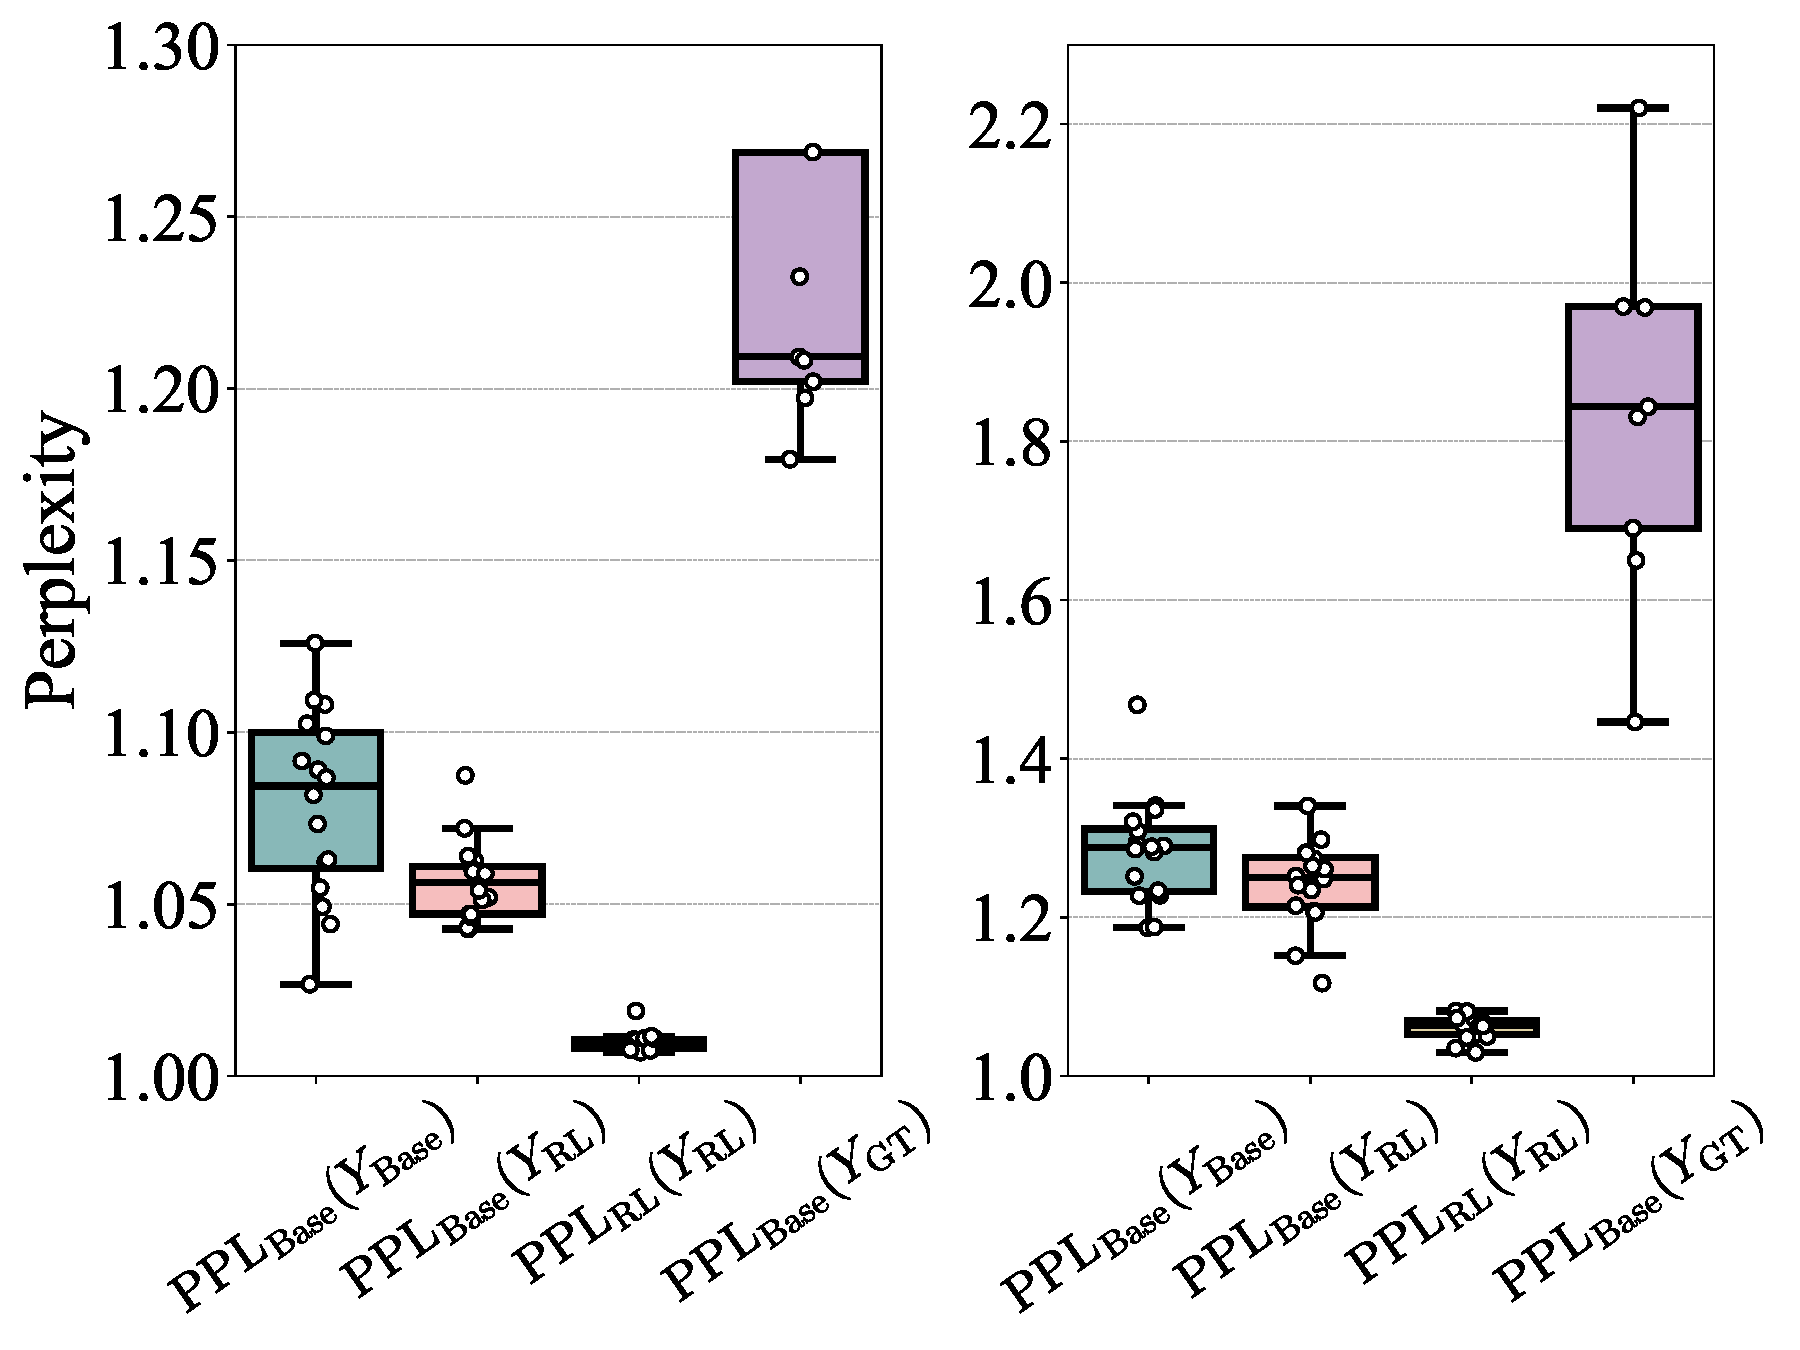
\includegraphics[width=\textwidth]{tex/images/box_plot_perplexity_aime24_combined_v2.pdf}
  \end{subfigure}
\captionsetup{font=footnotesize}
\caption{
Perplexity distribution of responses. The conditioning problem $x$ is omitted in the figure. 
}
\label{fig:perplexity}
\vspace{-6mm}
\end{wrapfigure}
We randomly sample two problems from AIME24 and employ Qwen2.5-7B-Base and SimpleRL-Qwen2.5-7B-Base to generate 16 responses for each problem, denoted as $\mathbf{Y}_\text{base}$ and $\mathbf{Y}_\text{RL}$, respectively. We also let OpenAI-o1~\cite{jaech2024openaio1} generate 8 responses, denoted as $\mathbf{Y}_\text{GT}$.
As shown in~\cref{fig:perplexity}, the distribution of $\text{PPL}_\text{Base} (\mathbf{Y}_\text{RL} | x)$ closely matches the lower portion of the $\text{PPL}_\text{Base} (\mathbf{Y}_\text{Base} | x)$ distribution, corresponding to responses that the base model tends to generate.  
This suggests that the responses from RL-trained models are highly likely to be generated by the base model. 
In~\cref{appendix:perplexity}, we show that $\text{PPL}_\text{Base} (\mathbf{Y}_\text{RL} | x)$ gradually decreases as RL training progresses, indicating that RLVR mainly sharpens the distribution within the base model's prior rather than expanding beyond it.

\textbf{Summary.} Combining the above analyses, we arrive at three key observations. First, problems solved by the RLVR model are also solvable by the base model; the observed improvement in average scores stems from more efficient sampling on these already solvable problems, rather than learning to solve new problems. Second, after RLVR training, the model often exhibits narrower reasoning coverage compared to its base model. Third, all the reasoning paths exploited by the RLVR model are already present in the sampling distribution of the base model. These findings indicate that RLVR does not introduce fundamentally new reasoning capabilities and that the reasoning capacity of the trained model remains bounded by that of its base model.

% \item \textbf{RLVR improves sampling efficiency.}
% Although the reasoning paths in the RL model already exist within the base model, RL training improves pass@1 performance, as shown by the left side of pass@$k$ curves. This indicates that by biasing the output distribution toward high-reward responses, RL increases the likelihood of sampling correct reasoning paths that are already encoded in the base model.

% \item \textbf{RLVR narrows the reasoning boundary.} The efficiency gain of RLVR comes at the expense of coverage: pass@$k$ decreases at larger $k$ values compared to the base model. We attribute this to the tendency of RL to reduce output entropy, which limits exploration~\cite{yu2025dapo}.


% \begin{figure}[t]
% \vspace{-1mm}
%   \centering
%   \begin{subfigure}[b]{0.475\textwidth}
%     \includegraphics[width=\textwidth]{tex/images/box_plot_perplexity_aime24_combined.pdf}
%   \end{subfigure}
%   % \begin{subfigure}[b]{0.15\textwidth}
%   %   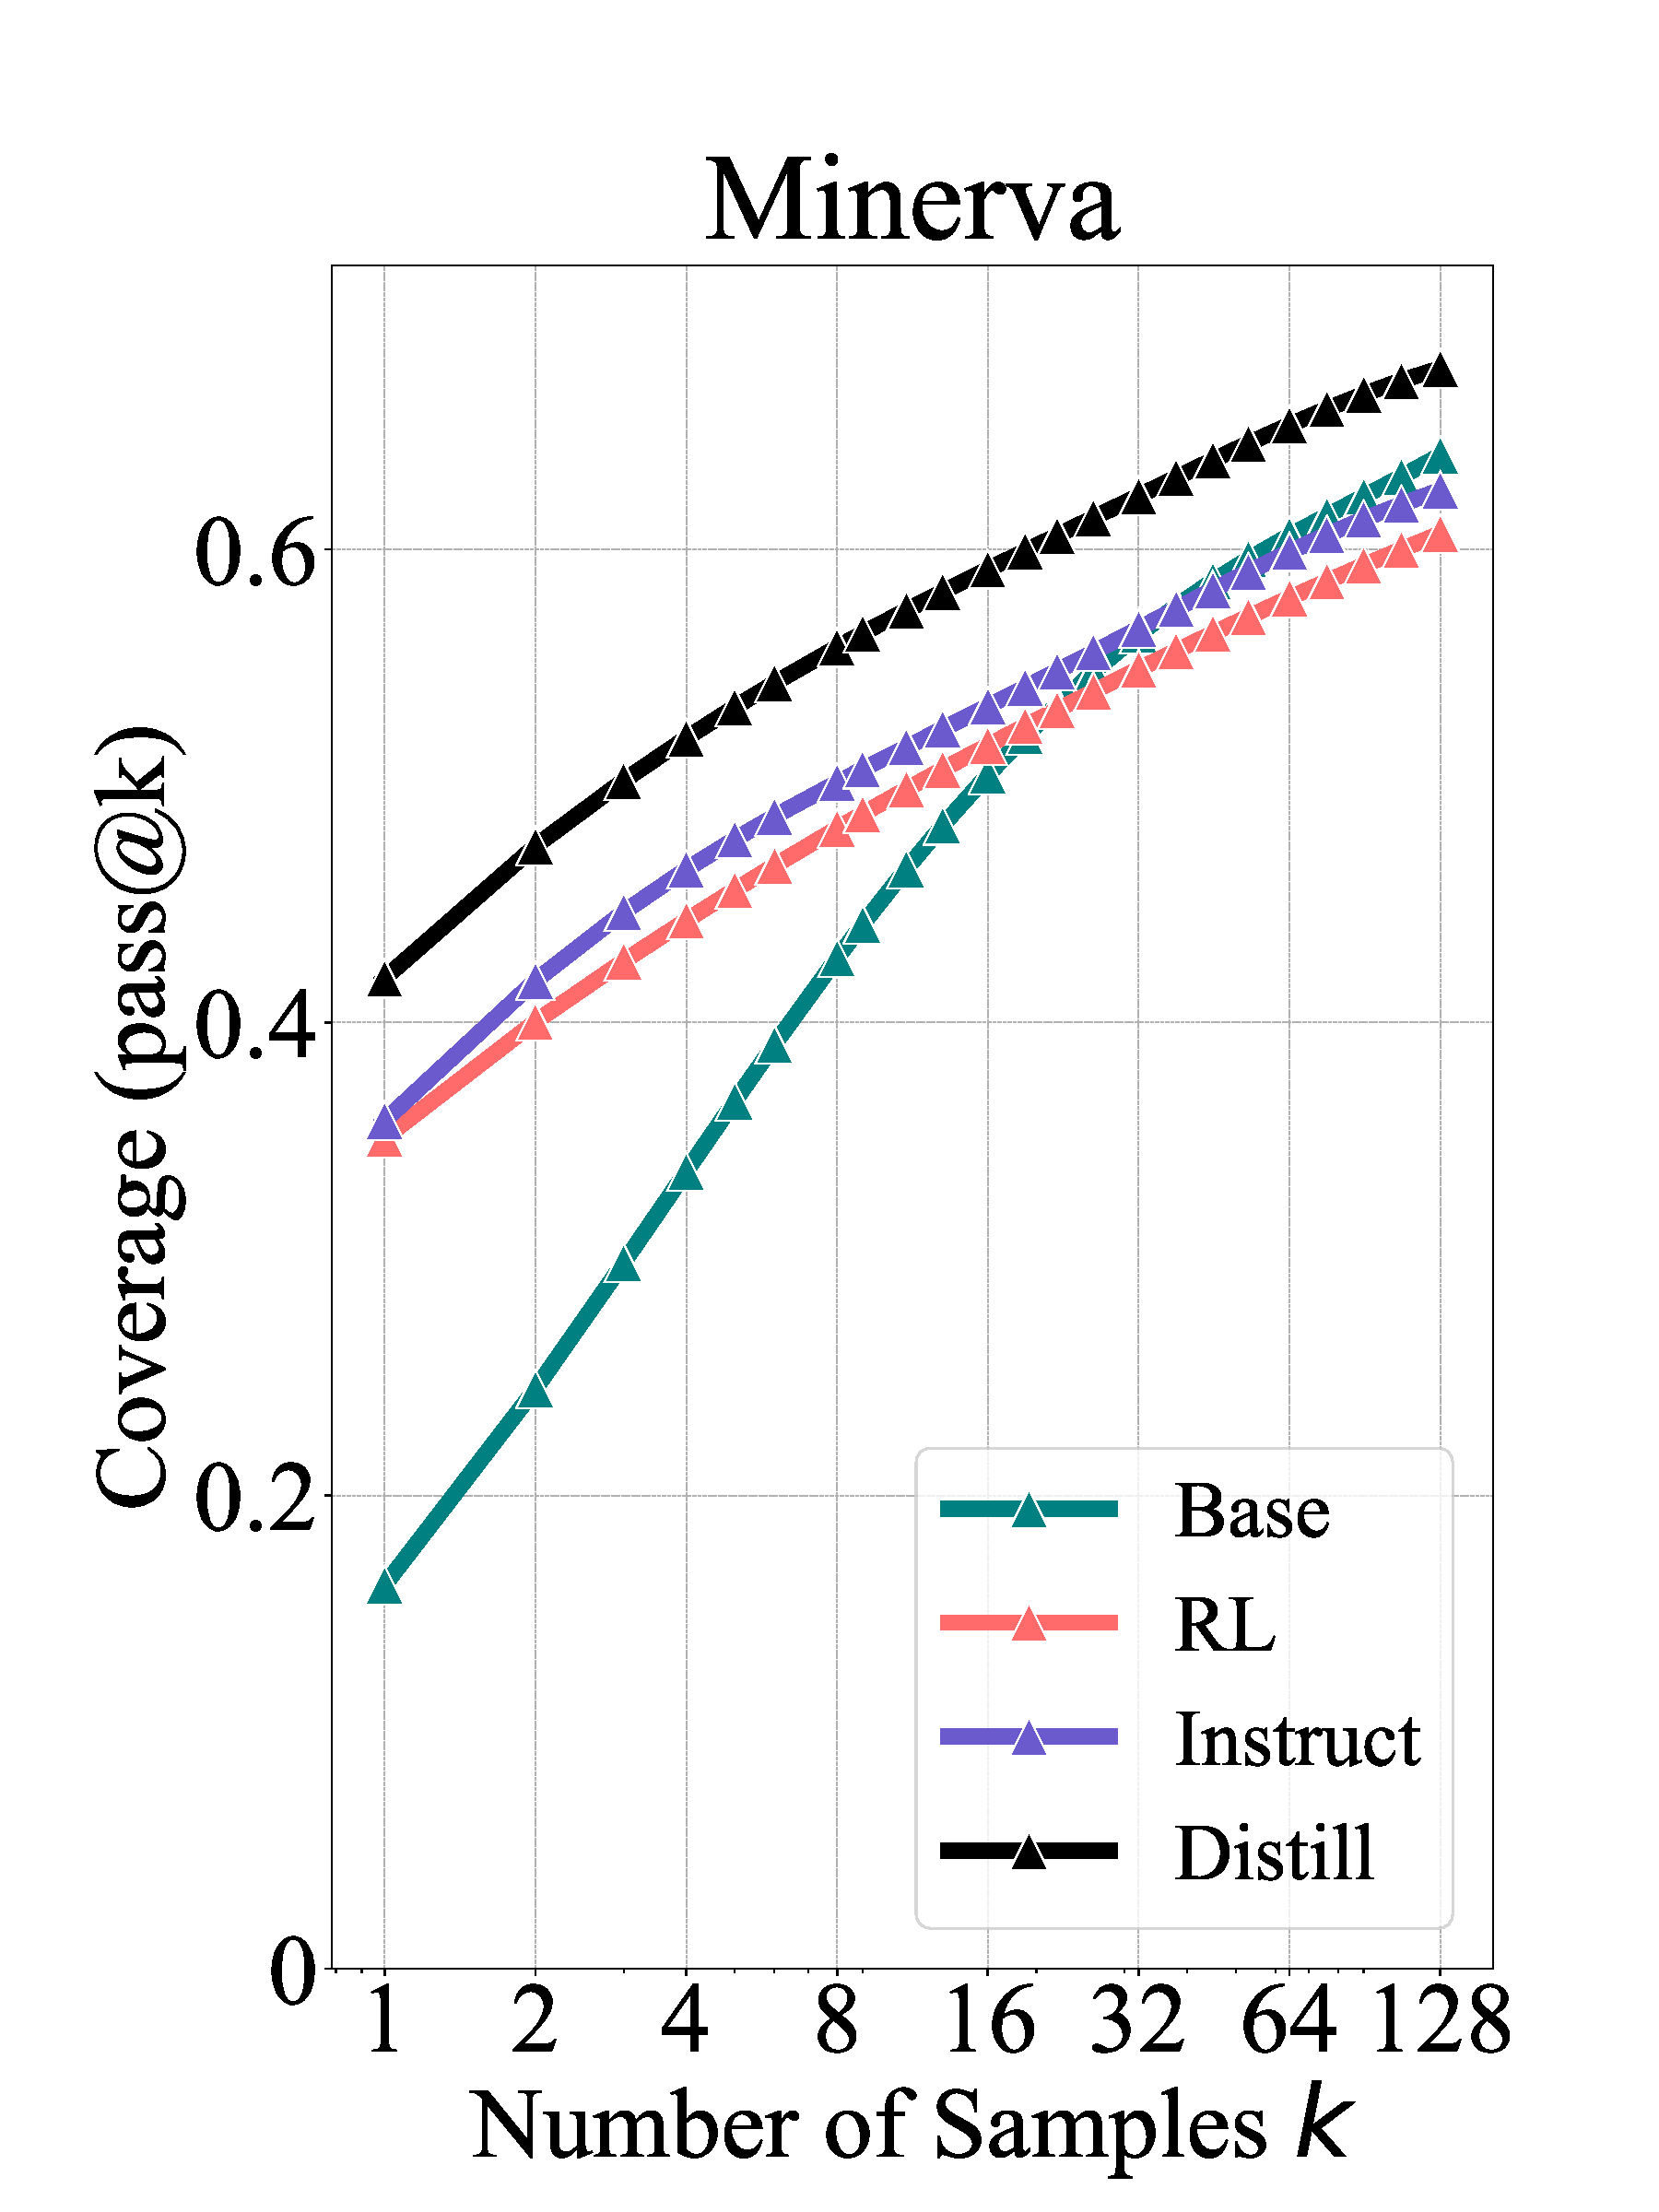
\includegraphics[width=\textwidth]{tex/images/distill_Minerva.pdf}
%   % \end{subfigure}
% \captionsetup{font=footnotesize}
% \caption{
% Perplexity distribution of responses. The conditioning problem $x$ is omitted in the figure. 
% % \textbf{Perplexity distribution of responses from different sources, evaluated by the base and RL models. The conditioning problem $x$ is omitted in the figure.  
% % \textbf{(Right)} Coverage comparison of base, Instruct, RL, and distilled models.
% }
% \label{fig:perplexity_and_distill}
% \vspace{-3mm}
% \end{figure}


\subsection{Distillation Expands the Reasoning Boundary}
\vspace{-1mm}

\begin{wrapfigure}{r}{0.235\textwidth}
\vspace{-4mm}
  \centering
  \begin{subfigure}[b]{0.235\textwidth}
    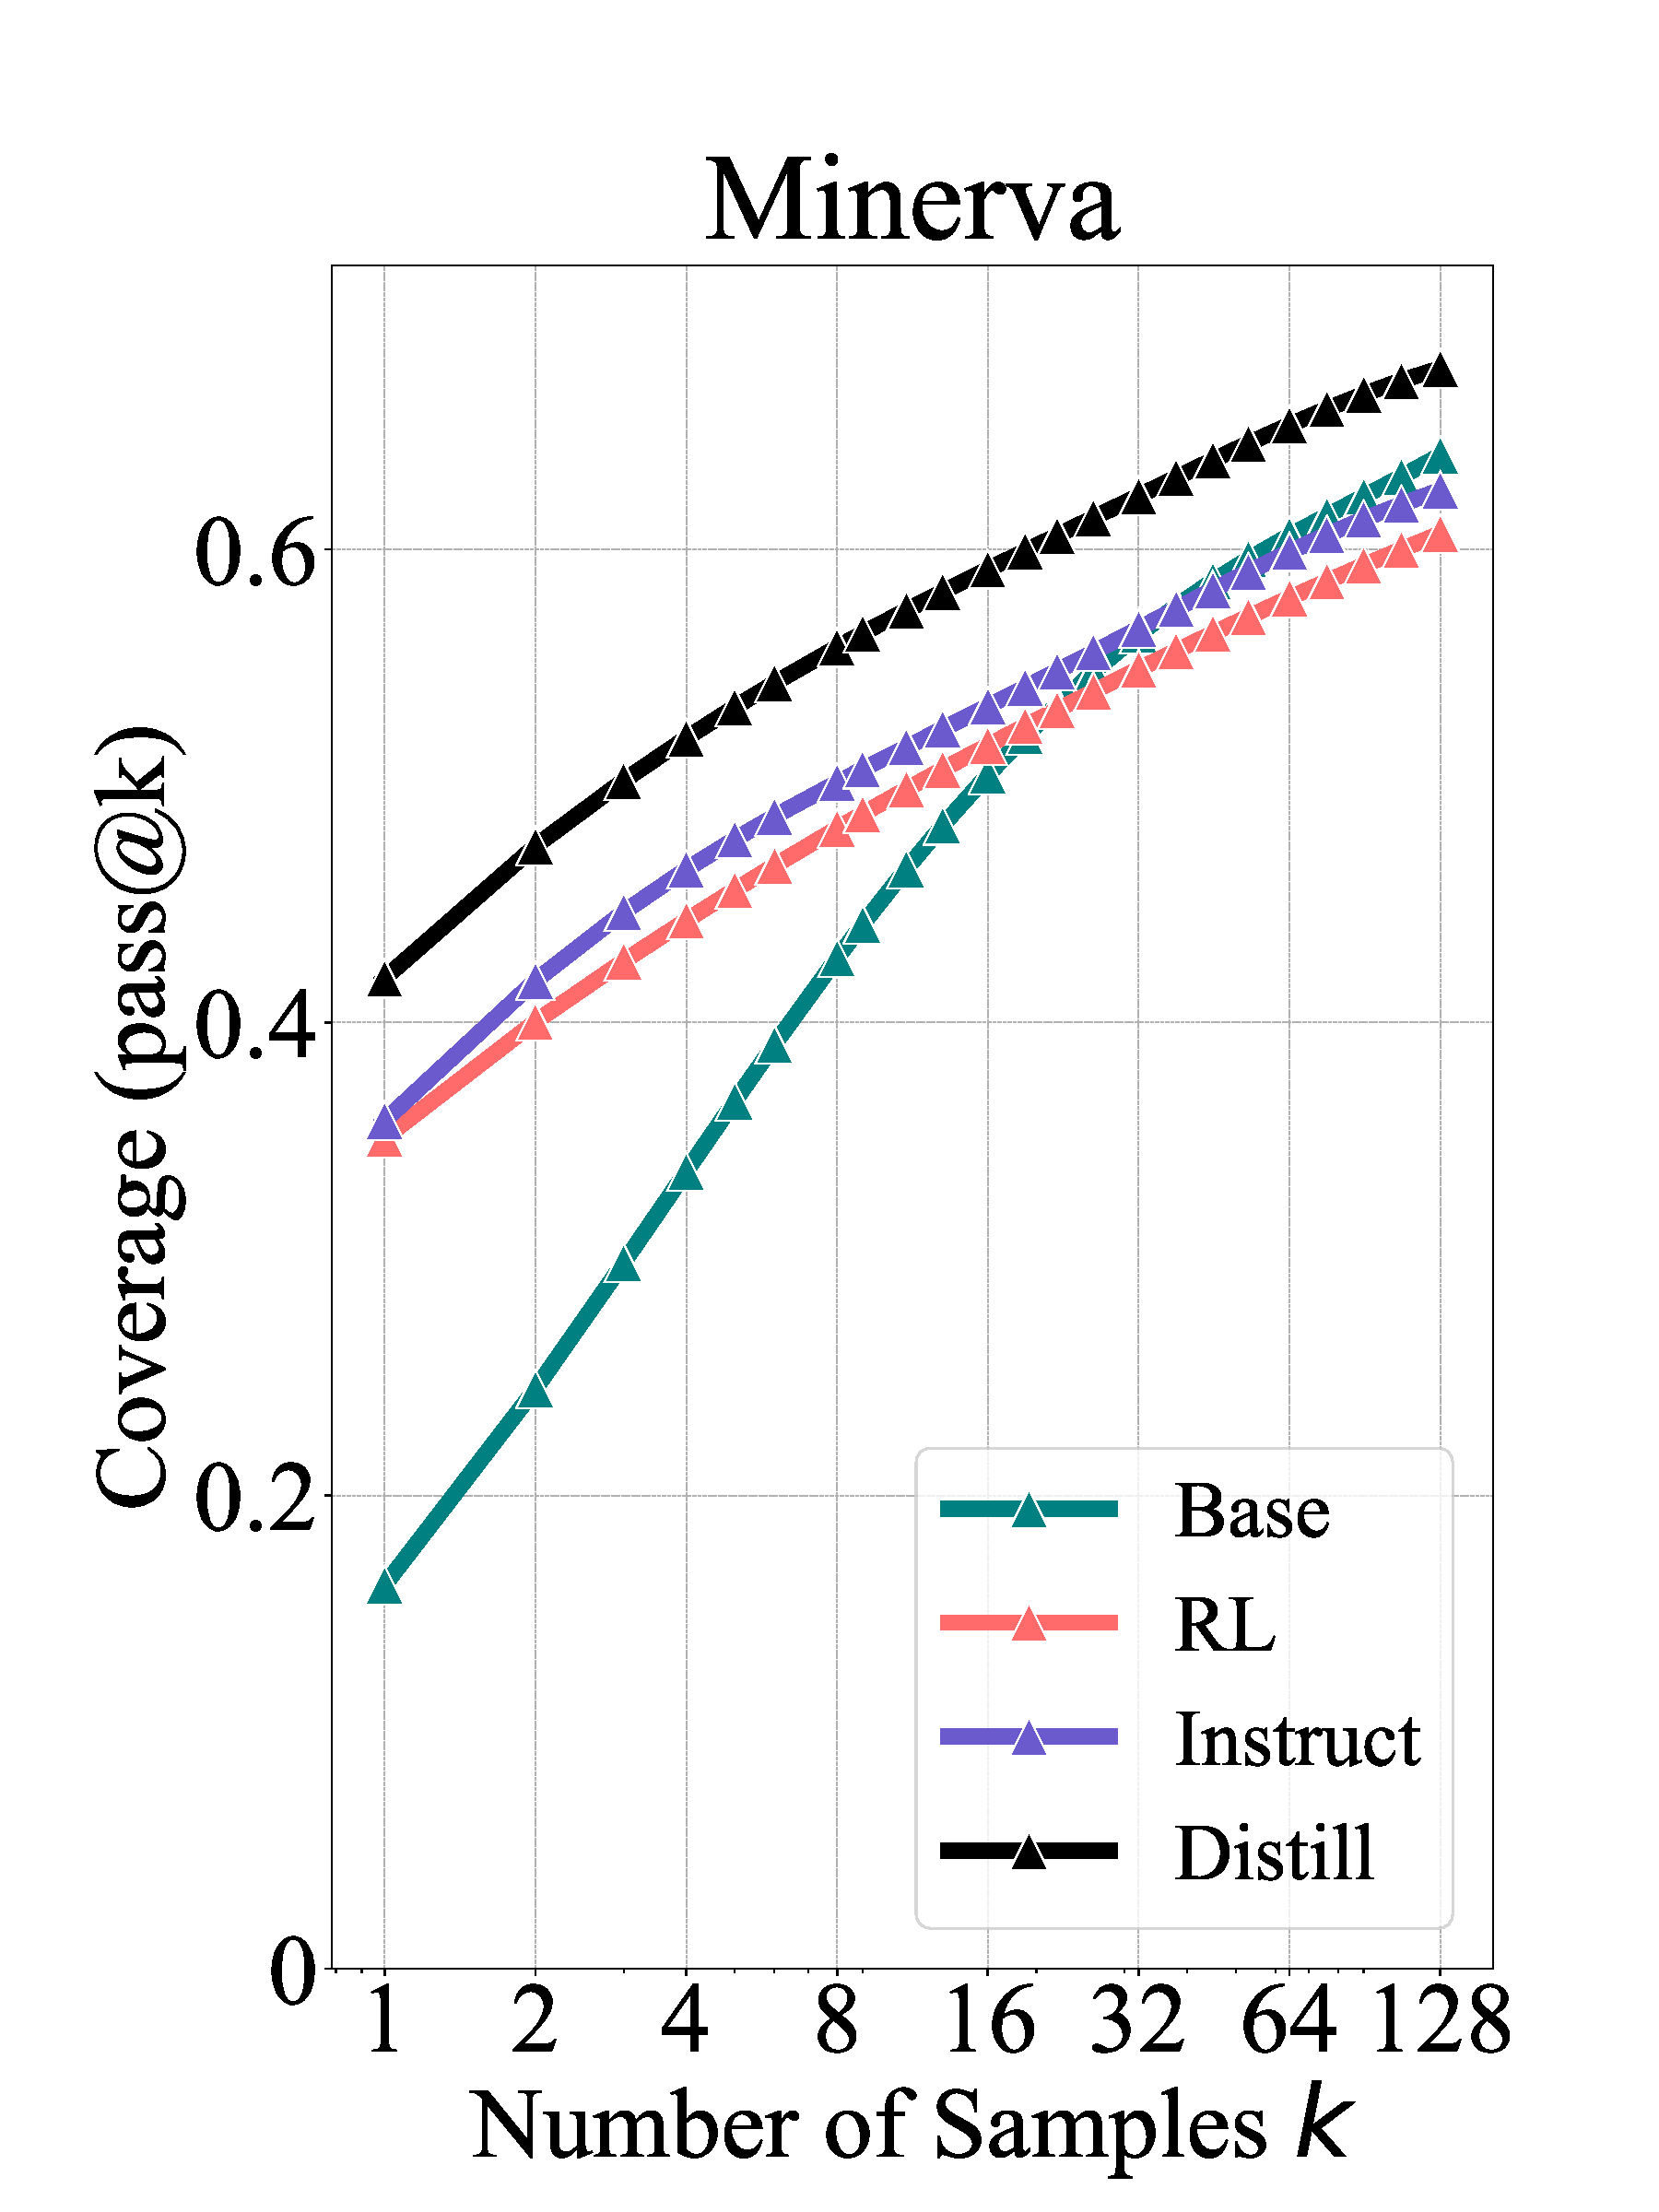
\includegraphics[width=\textwidth]{tex/images/distill_Minerva.pdf}
  \end{subfigure}
\captionsetup{font=footnotesize}
\caption{
pass@$k$ of base, Instruct, RLVR, and distilled models.
}
\label{fig:distill}
\vspace{-4mm}
\end{wrapfigure}
In addition to direct RL training, another effective approach to improving the reasoning ability of small base models is distillation from a powerful reasoning model~\cite{guo2025deepseek-r1}.  
This process is analogous to instruction-following fine-tuning in post-training. 
However, instead of using short instruction-response pairs, the training data consist of long CoT reasoning traces generated by the teacher model.
Given the limitations of current RLVR in expanding reasoning capabilities, it is natural to ask whether distillation exhibits similar behavior.
We focus on a representative model, DeepSeek-R1-Distill-Qwen-7B, which distills DeepSeek-R1 into Qwen2.5-Math-7B.  
We compare it with the base model Qwen2.5-Math-7B and its RL-trained counterpart Qwen2.5-Math-7B-Oat-Zero and include Qwen2.5-Math-7B-Instruct as an additional baseline.
As shown in~\cref{fig:distill}, the pass@$k$ curve of the distilled model is consistently and significantly above that of the base model.  
This indicates that, unlike RL that is fundamentally bounded by the reasoning capacity of the base model, distillation introduces new reasoning patterns learned from a stronger teacher model. As a result, the distilled model is capable of surpassing the reasoning boundary of the base model.

% \begin{figure}[t]
%   \centering
%   \begin{subfigure}[b]{0.98\textwidth}
%     \includegraphics[width=\textwidth]{tex/images/qwen25_7b_base_algo_coverage_broken_yaxis_v2.pdf}
%   \end{subfigure}
% \captionsetup{font={footnotesize}}
% \caption{
% \textbf{Different RL algorithms.}
% % \textbf{(Bottom)} Different RL training steps.
% We use a \textit{folded y-axis} range to better highlight the details at $k=1$ and $256$.
% Unfolded version can be found in~\cref{fig:algo_and_step_unfold}.
% The detailed values for each point at pass@1 and pass@256 are provided in~\cref{tab:algos} and~\cref{tab:grpo_training_steps}.
% }
% \label{fig:algo_and_step}
% \vspace{-3mm}
% \end{figure}

\subsection{Effects of Different RL Algorithms}
\vspace{-1mm}
\label{sec:algos}

As discussed previously, the primary effect of RL is to enhance sampling efficiency rather than to expand a model's reasoning capacity.  
To quantify this, we propose the \textit{Sampling Efficiency Gap} ($\Delta_{\text{SE}}$), defined as the difference between the RL-trained model's pass@1 and the base model's pass@$k$ (we use $k = 256$ in our evaluation). 
Lower $\Delta_{\text{SE}}$ is better.
Here we conduct clean experiments to study the effect of different RL algorithms in enhancing sampling efficiency.

\textbf{Experiment Setup.}
We re-implement popular RL algorithms using the VeRL framework~\cite{sheng2024verl} for fair comparison, including PPO~\cite{schulman2017ppo}, GRPO~\cite{shao2024deepseekmath}, Reinforce++~\cite{hu2025reinforce++}, RLOO~\cite{ahmadian2024rloo}, ReMax~\cite{li2023remax}, and DAPO~\cite{yu2025dapo}.
Following DAPO~\cite{yu2025dapo} and Oat-Zero~\cite{liu2025oat}, we remove the KL term to avoid constraining model learning. 
During training, we use the AdamW optimizer~\cite{adamw} with a constant learning rate of $10^{-6}$. For rollout, we employ a prompt batch size of 256 and generate 8 responses per prompt. The maximum rollout length is set to 8,192 tokens, and the sampling temperature is set as 1.0. We use a PPO mini-batch size of 256.

To assess in-domain and out-of-domain generalization under RLVR, we split Omni-MATH-Rule, a subset of Omni-MATH~\cite{gao2024omnimathuniversalolympiadlevel} containing verifiable problems, into a training set (2,000 samples) and an in-domain test set (821 samples), and use MATH500 as the out-of-domain benchmark. 
% All algorithms are trained using 150 steps.

\textbf{Results.}
As shown in~\cref{fig:algo_and_step} (top), although different RL algorithms exhibit slight variations in both pass@1 and pass@256, these differences are not fundamental.  
Different RL algorithms yield slightly different $\Delta_{\text{SE}}$ values (\ie, ranging from GRPO's 43.9 to RLOO's best 42.6 on the in-domain test set).  
Furthermore, we observe that $\Delta_{\text{SE}}$ remains consistently above 40 points across different algorithms, highlighting that existing RL methods are still far from achieving optimal sampling efficiency. This suggests that novel RL algorithms or entirely new paradigms may be necessary to approach the upper bound. Additional observations can be found at~\cref{appendix:algos}.


\begin{figure}[!t]
\vspace{-1mm}
  \centering
  \begin{subfigure}[b]{0.92\textwidth}
    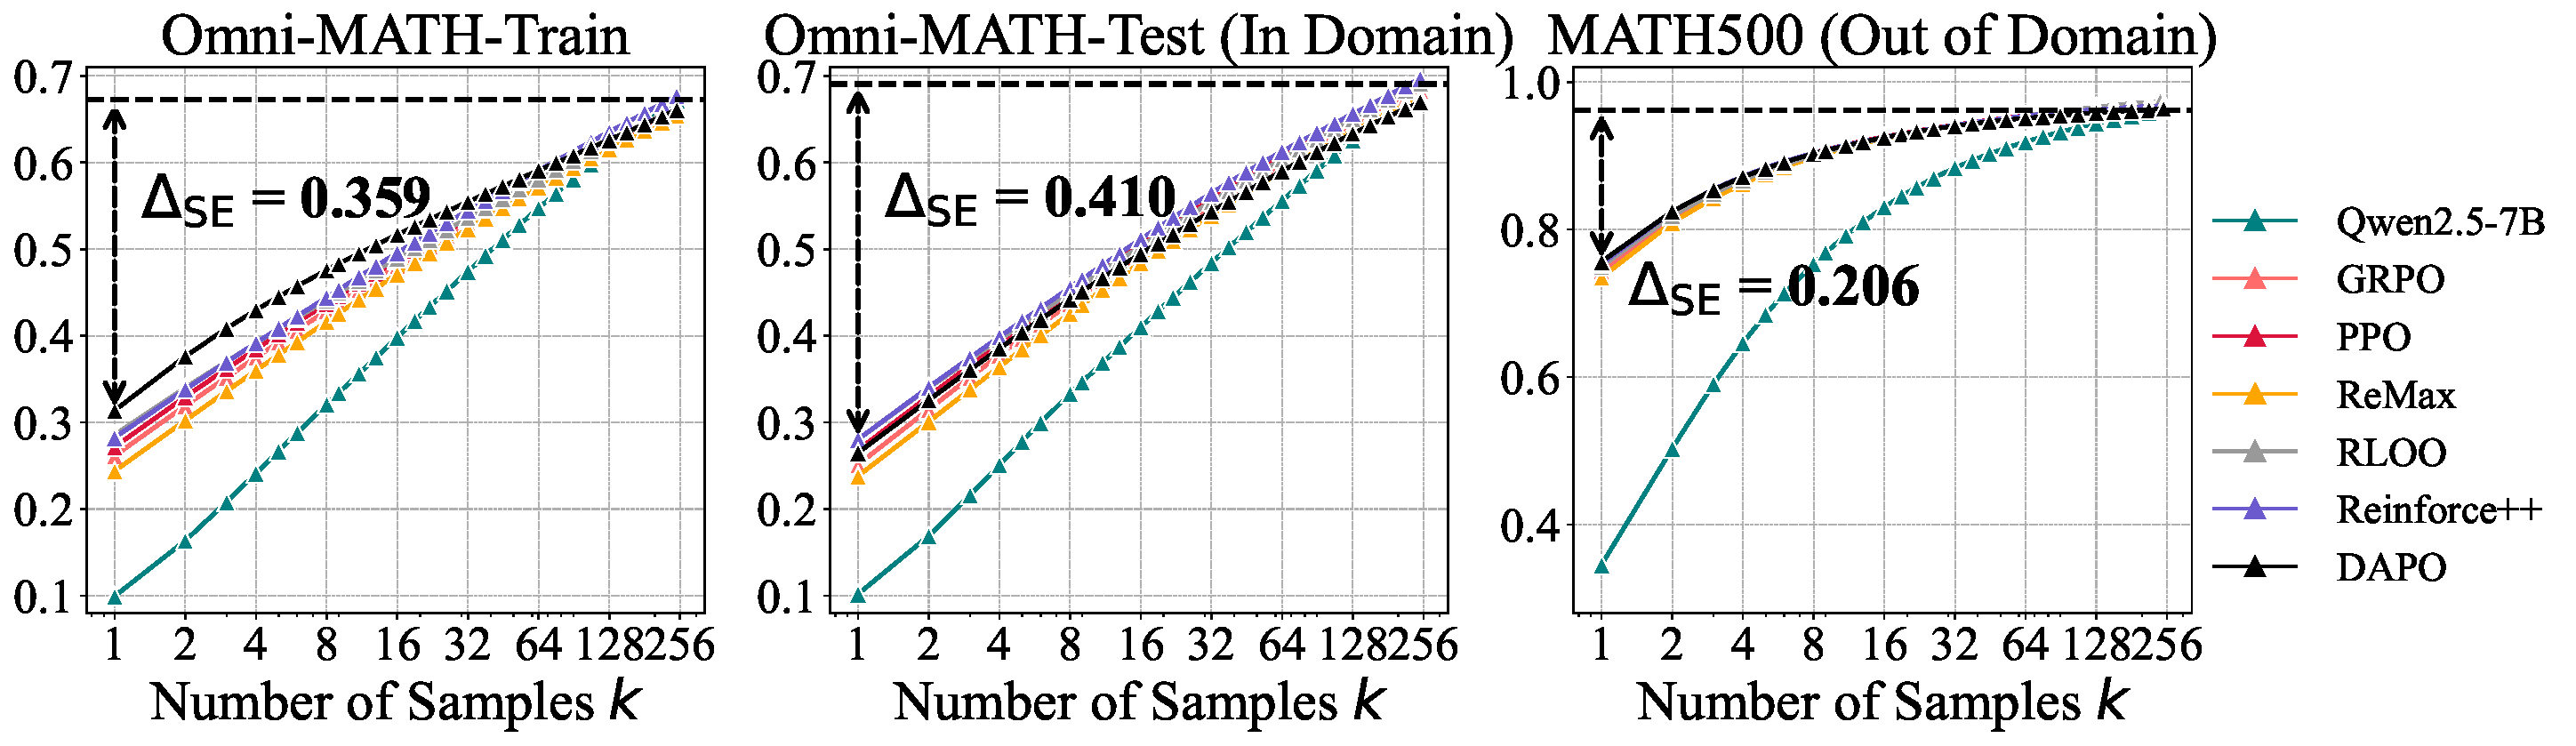
\includegraphics[width=\textwidth]{tex/images/qwen25_7b_base_algo_coverage_final.pdf}
  \end{subfigure}
  \begin{subfigure}[b]{0.92\textwidth}
    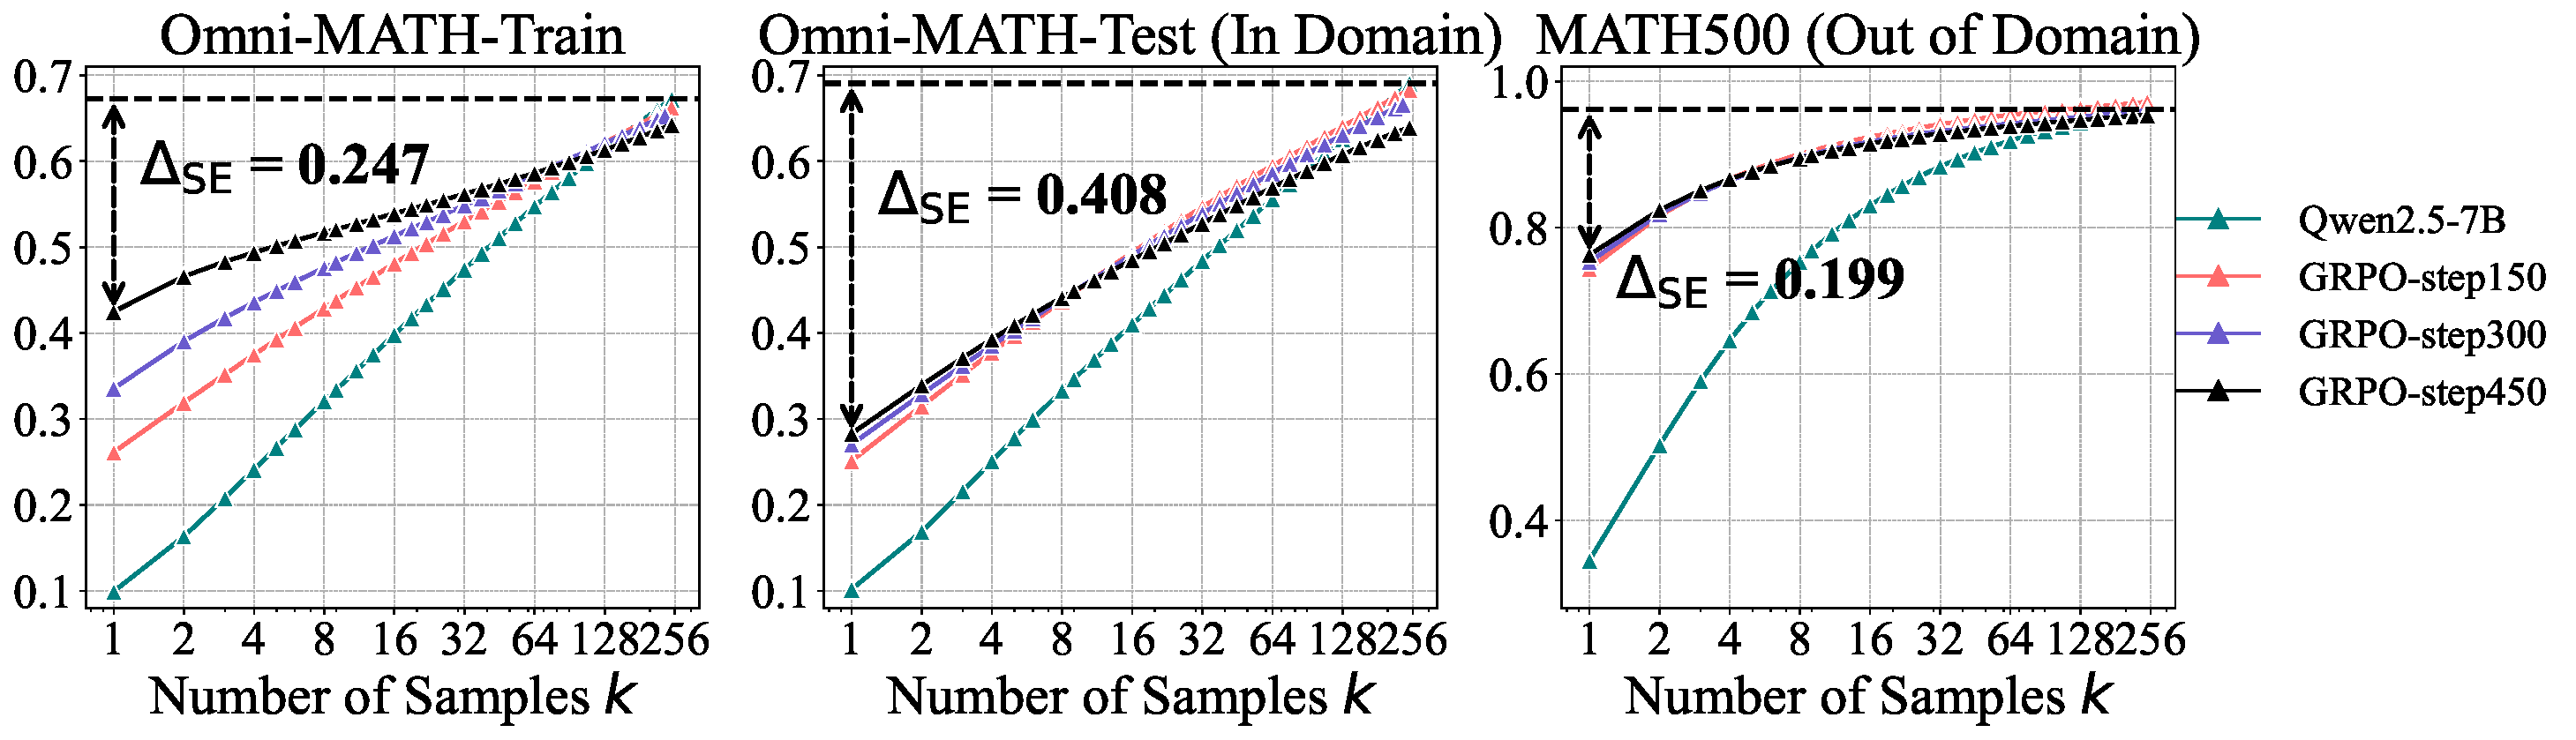
\includegraphics[width=\textwidth]{tex/images/qwen25_7b_base_step_coverage_final.pdf}
  \end{subfigure}
% \captionsetup{font={footnotesize}}
\caption{
\textbf{(Top)} Different RL algorithms.
\textbf{(Bottom)} Different RL training steps.
The detailed values for each point at pass@1 and pass@256 are provided in~\cref{tab:algos} and~\cref{tab:grpo_training_steps}.
}
% \label{fig:algo_and_step_unfold}
\label{fig:algo_and_step}
\vspace{-4mm}
\end{figure}



\vspace{-0.5mm}
\subsection{Effects of RL Training}
\vspace{-0.5mm}
\label{sec:steps}

\textbf{Asymptotic Effects.}
Based on the setup in~\cref{sec:algos}, we investigate the effect of the training steps on the asymptotic performance of the model. As shown in~\cref{fig:overview} (right), as RL training progresses, pass@1 on the training set consistently improves from 26.1 to 42.5. 
% However, several observations suggest that longer training may not yield substantial benefits.
% First, we observe that \textit{pass@1} after 450 steps on both in-domain and out-of-domain test sets shows only a marginal improvement compared to 150 steps, much smaller than the gain observed in the training set. 
% This suggests that RL training might be overfitting the training set to some degree.
However, as RLVR training progresses, pass@256 progressively decreases, indicating a reduced reasoning boundary. 
% This is likely because, as RL training progresses, the model's output entropy and exploration ability decrease.

\textbf{Effect of Number of Rollouts $n$.} 
The training hyperparameter $n$, the number of responses per prompt, can affect pass@$k$ by enabling broader exploration during training. We increase $n$ from 8 to 32. As shown in~\cref{fig:grpo_ablate}, pass@$k$ improves slightly over $n=8$, but the RL-trained model is still eventually outperformed by the base model. 
% This suggests that scaling up RL alone may not be sufficient to surpass the base model's reasoning capacity.
We leave the question of whether scaling RLVR training can eventually surpass the base model to future investigation.


\textbf{Effect of KL Loss.} 
To control model deviation, some prior work adds a KL penalty. We ablate this by applying a KL term with coefficient 0.001. As shown in~\cref{fig:grpo_ablate}, the KL-regularized model achieves similar pass@1 to GRPO without KL, but with a much lower pass@128.

\vspace{-0.5mm}
\subsection{Effects of Entropy}
\vspace{-0.5mm}

As RL training progresses, the model's output entropy typically decreases~\cite{yu2025dapo}, which may contribute to a reduced reasoning boundary due to less diverse output. 
To investigate this factor, we increase the generation temperature of the RLVR-trained model to match the output entropy of the base model at $T = 0.6$. 
As shown in~\cref{fig:equal_entropy}, although the RLVR model performs slightly better pass@$k$ at higher temperatures compared to its own performance at $T = 0.6$, it still underperforms the base model across pass@$k$.
This suggests that while reduced entropy contributes to the narrowing of the reasoning boundary, it alone does not fully account for the reduction.


\vspace{-0.5mm}
\subsection{Effects of Model Size Scaling}
\vspace{-0.5mm}

Scaling plays a central role in the capabilities of contemporary LLMs. It remains an important question whether the conclusions drawn continue to hold as model size increases. 
For many large models, isolating the effect of RLVR is not feasible. For example, in the case of GPT-o1, the base model is not publicly accessible. Qwen3-235B~\cite{yang2025qwen3} is trained through multiple stages, including RLVR and long-context CoT supervised fine-tuning, which makes it impossible to disentangle the impact of RLVR alone. For Deepseek-R1-Zero, the absence of a publicly hosted API forced us to self-host the model, but throughput was limited to around 50 tokens per second at a maximum sequence length of 32k, rendering pass@$k$ evaluation currently impractical.
As a more tractable alternative, we selected the Magistral-Medium-2506 API to conduct a preliminary set of experiments.
This model is trained using pure RL, with Mistral-Medium-3-2505 as the starting model~\cite{rastogi2025magistral}. Although the model size is not disclosed, Magistral-Medium performs comparably to Deepseek-R1 and is positioned near the frontier in terms of reasoning capability.


\begin{wrapfigure}{r}{0.56\textwidth}
\vspace{-2mm}
  \centering
  \begin{subfigure}[b]{0.275\textwidth}
    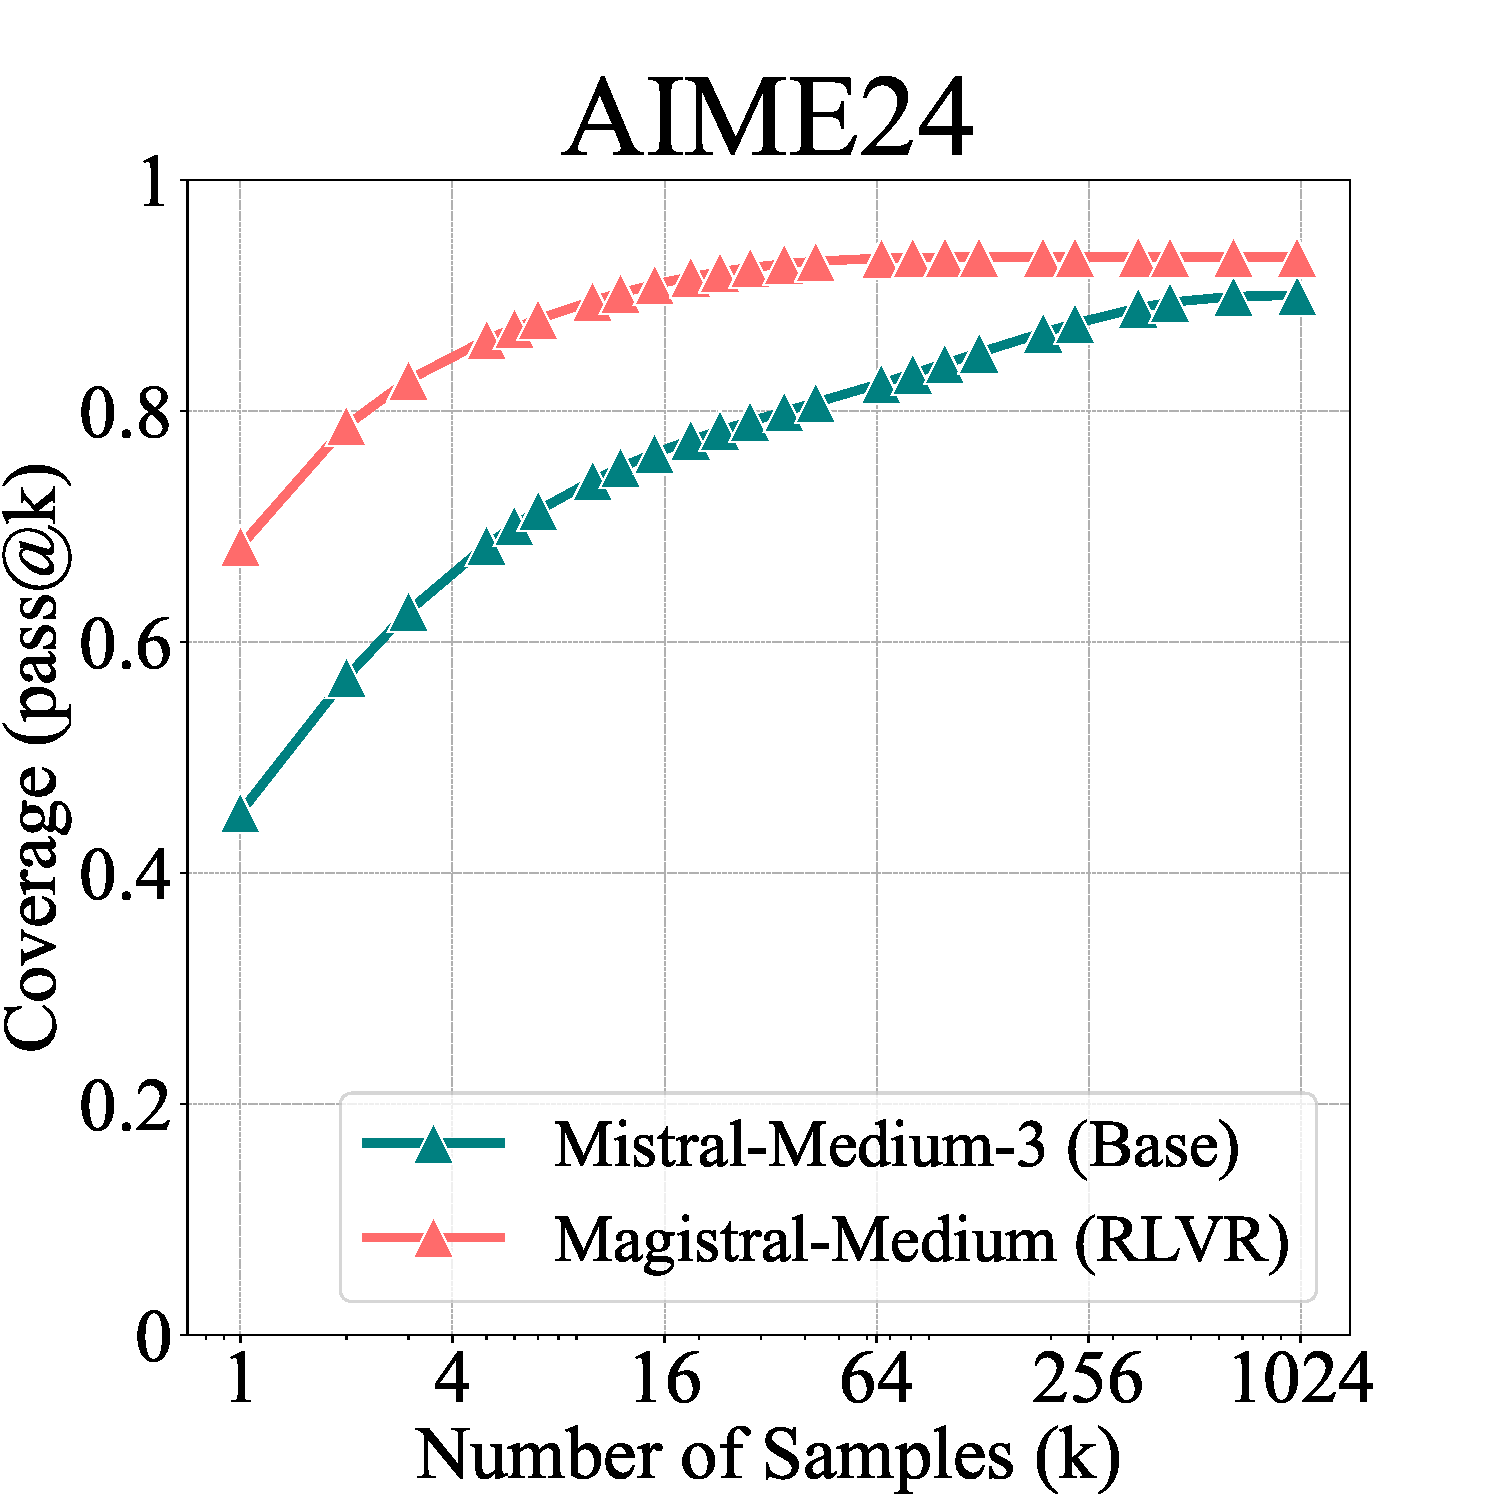
\includegraphics[width=\textwidth]{tex/images/simpleRL_coverage_magistral_24-final.pdf}
  \end{subfigure}
  \begin{subfigure}[b]{0.275\textwidth}
    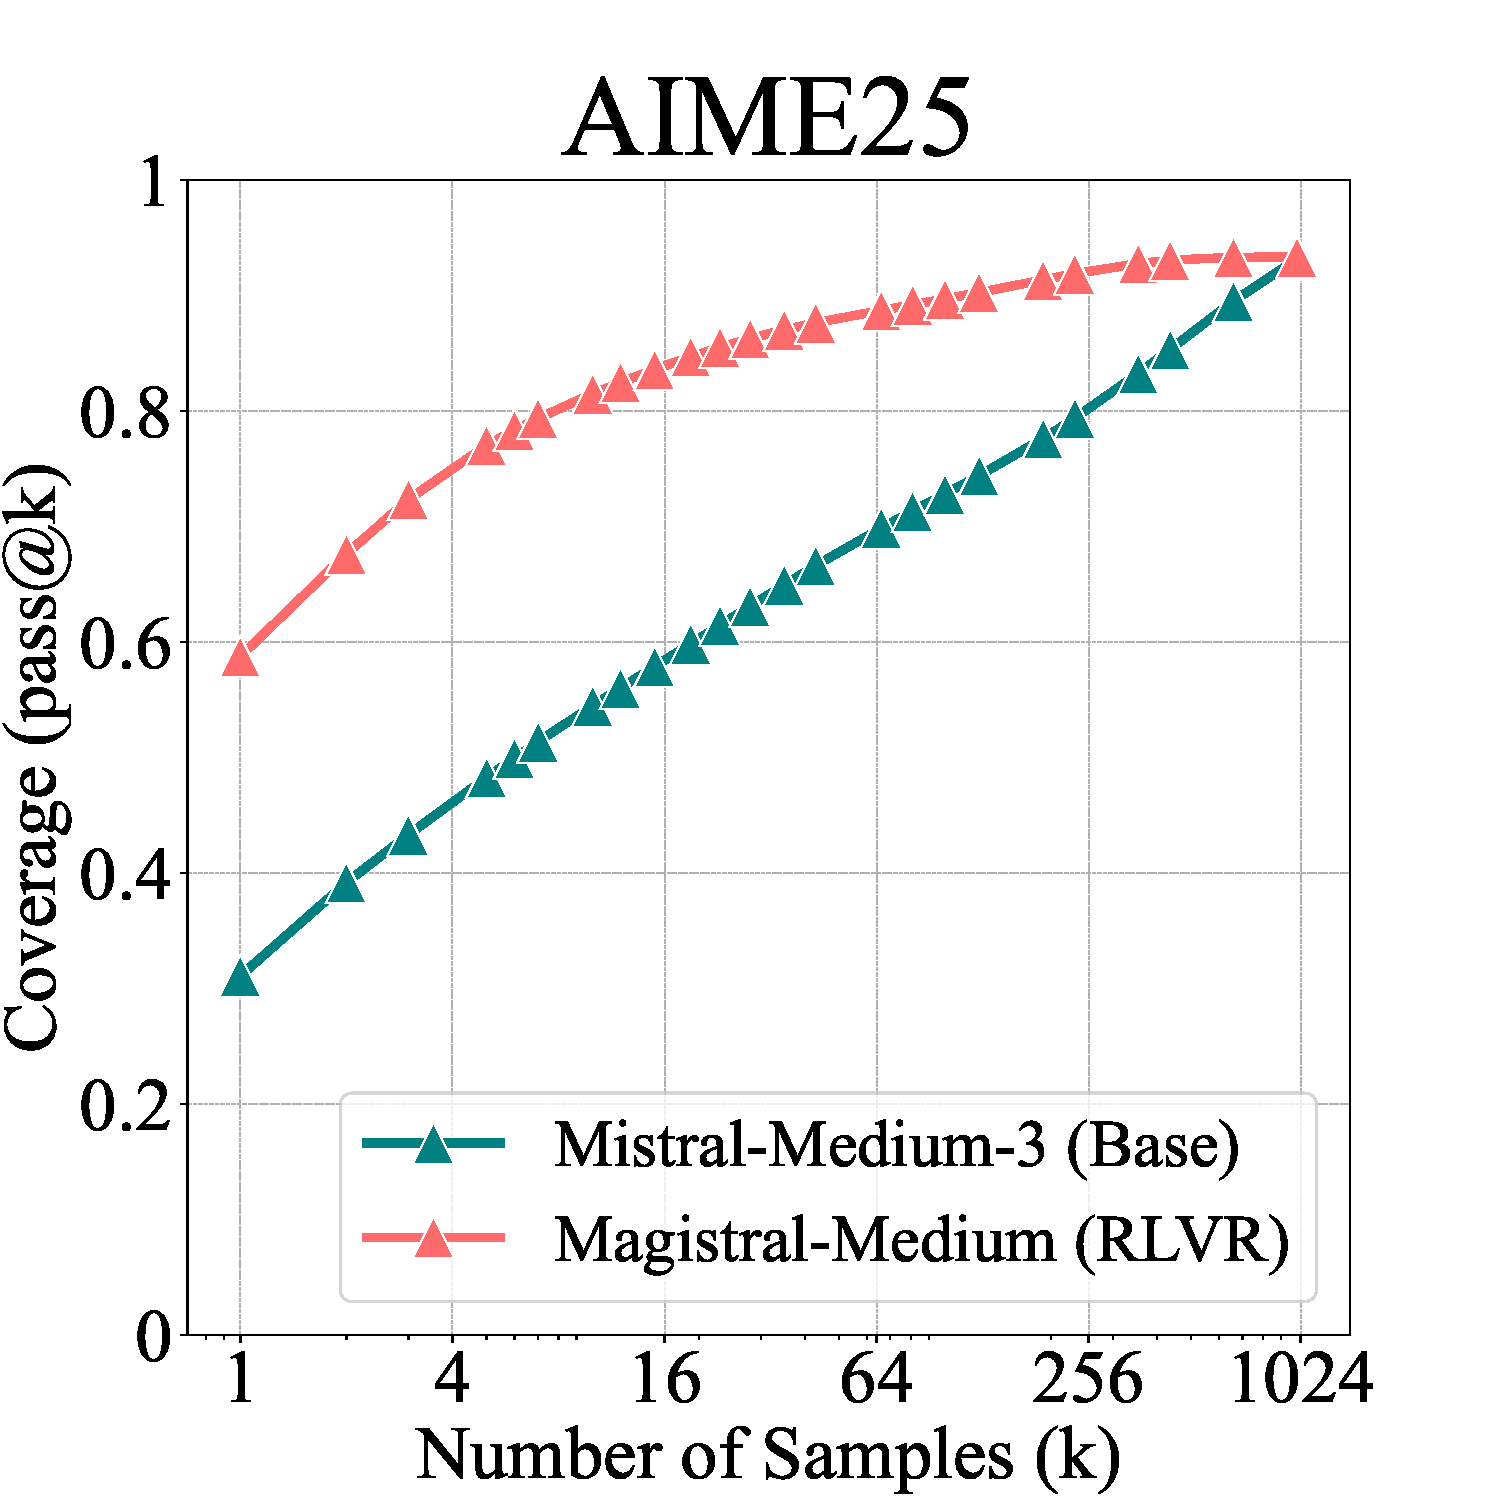
\includegraphics[width=\textwidth]{tex/images/simpleRL_coverage_magistral_25-final.pdf}
  \end{subfigure}
\captionsetup{font=footnotesize}
\caption{
pass@$k$ curves of Magistral-Medium.
}
\label{fig:magistral}
\vspace{-2mm}
\end{wrapfigure}
We queried the models using a maximum context length of 40k as the original paper does. Once again, we observed that RLVR provides significant gains at low $k$, but little or no improvement at higher $k$. Specifically, at $k = 1$, the RLVR-enhanced model solves approximately 7 more problems on AIME24 and 8 more on AIME25 compared to its base version. However, as $k$ increases, the performance gap steadily narrows.
% These observations suggest that our conclusion continues to hold even for highly capable, frontier-level reasoning models.
% It's a to investigate if it holds in the future if more compute such as the aomount of pretrain is used for RL training.
These observations suggest that our conclusion continues to hold even for current, highly capable, near-frontier reasoning models. 
Whether this trend persists as more compute, such as pre-training scale budgets, is dedicated to RL training remains a critical question for the future of LLM reasoning.
